\documentclass{beamer}

\usepackage[utf8]{inputenc}
\usepackage{tikz}

\title{Multilayer Perceptron}
\subtitle{Multilayer Dense Feedforward Neural Networks}
\author{Vitor Greati\inst{1}}
\institute[]
{
	\inst{1}%
	Federal University of Rio Grande do Norte
}
\date{}
\subject{Computer Science}

% Table of contents at the beginning of each section
\AtBeginSection[]
{
  \begin{frame}
    \frametitle{Table of Contents}
    \tableofcontents[currentsection]
  \end{frame}
}

% Table of contents at the beginning of each subsection
%\AtBeginSubsection[]
%{
%  \begin{frame}
%    \frametitle{Table of Contents}
%    \tableofcontents[currentsection,currentsubsection]
%  \end{frame}
%}

\begin{document}

\frame{\titlepage}

\section{Introduction}

    \begin{frame}{Introduction}
        TODO.
    \end{frame}

    \subsection{Neurons}


    \begin{frame}{Neurons}{Basic elements}

        The neuron's basic task is to take an input, perform some computation and
        output a value.

        \begin{block}{Main elements}
            \begin{itemize}
                \item An input vector $\mathbf{x} = \langle x_1, x_2, \ldots, x_n \rangle \in \mathbb{R}^n$.
                \item A vector of weights $\mathbf{w} = \langle w_1, w_2, \ldots, w_n \rangle \in \mathbb{R}^n$.
                \item A constant $b \in \mathbb{R}$, called \emph{bias}.
                \item A computation between inputs and weights, like 
                    $$z=\mathbf{x}\cdot\mathbf{w} =\sum_i x_iw_i.$$
                \item An activation function $f$ to produce an output $f(z + b)$.
            \end{itemize}
        \end{block}
    \end{frame}

    \begin{frame}{Neurons}{Graphical representation}
        A common graphical representation highlights those elements:
        \begin{figure}
            \centering
            \begin{tikzpicture}
                \draw (4,1) node[circle,minimum size=3cm,draw] (A) {};
                \node (B) at (0,3) {$x_1$};
                \node (C) at (0,2) {$x_2$};
                \node (D) at (0,1) {$x_3$};
                \node (E) at (0,0) {$\vdots$};
                \node (F) at (0,-1) {$x_n$};
                \draw [->] (B) -- (A);
                \draw [->] (C) -- (A);
                \draw [->] (D) -- (A);
                \draw [->] (F) -- (A);
                \node (H) at (8,1) {$a=f(z+b)$};
                \draw [->] (A) -- (H);
                \node (G) at (4,1) {$z=\sum_i x_iw_i$};
            \end{tikzpicture}
        \end{figure}
    \end{frame}

    \begin{frame}{Neurons}{Graphical representation}
        The same representation, but using only vectors:

        \begin{figure}
            \centering
            \begin{tikzpicture}
                \draw (4,1) node[circle,minimum size=3cm,draw] (A) {};
                \node (D) at (0,1) {$\mathbf x$};
                \draw [->] (D) -- (A);
                \node (H) at (8,1) {$a=f(z+b)$};
                \draw [->] (A) -- (H);
                \node (G) at (4,1) {$z=\mathbf{x} \cdot \mathbf{w}$};
            \end{tikzpicture}
        \end{figure}
    \end{frame}

    \subsection{Multilayer Architecture}

        \begin{frame}{Multilayer Architecture}{Dense feedfoward architecture}
            
            An architecture with $k$ layers, $L_0, L_1, \ldots, L_{k-1}$,
            is graphically represented as:

            \begin{figure}
                \centering
                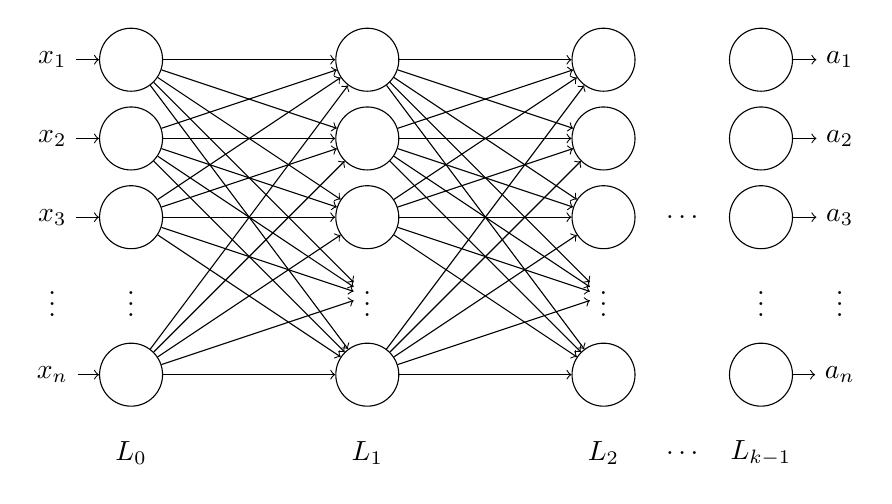
\begin{tikzpicture}
                    % Layer 1
                    \draw (0,4) node[circle,minimum size=0.8cm,draw] (A1) {};
                    \draw (0,3) node[circle,minimum size=0.8cm,draw] (A2) {};
                    \draw (0,2) node[circle,minimum size=0.8cm,draw] (A3) {};
                    \node (A) at (0,1) {$\vdots$};
                    \draw (0,0) node[circle,minimum size=0.8cm,draw] (A4) {};
                    \node (AL) at (0,-1) {$L_0$};
                    % Ins
                    \node (I1) at (-1,4) {$x_1$};
                    \draw [->](I1) -- (A1);
                    \node (I2) at (-1,3) {$x_2$};
                    \draw [->](I2) -- (A2);
                    \node (I3) at (-1,2) {$x_3$};
                    \draw [->](I3) -- (A3);
                    \node (I) at (-1,1) {$\vdots$};
                    \node (I4) at (-1,0) {$x_n$};
                    \draw [->](I4) -- (A4);
                    % Layer 2
                    \draw (3,4) node[circle,minimum size=0.8cm,draw] (B1) {};
                    \draw (3,3) node[circle,minimum size=0.8cm,draw] (B2) {};
                    \draw (3,2) node[circle,minimum size=0.8cm,draw] (B3) {};
                    \node (B) at (3,1) {$\vdots$};
                    \draw (3,0) node[circle,minimum size=0.8cm,draw] (B4) {};
                    \node (BL) at (3,-1) {$L_1$};
                    % Layer 3
                    \draw (6,4) node[circle,minimum size=0.8cm,draw] (C1) {};
                    \draw (6,3) node[circle,minimum size=0.8cm,draw] (C2) {};
                    \draw (6,2) node[circle,minimum size=0.8cm,draw] (C3) {};
                    \node (C) at (6,1) {$\vdots$};
                    \draw (6,0) node[circle,minimum size=0.8cm,draw] (C4) {};
                    \node (CL) at (6,-1) {$L_2$};
                    % Layers 4..k-1
                    \node (DDD1) at (7,2) {$\ldots$};
                    \node (DDD2) at (7,-1) {$\ldots$};
                    % Layer k
                    \draw (8,4) node[circle,minimum size=0.8cm,draw] (D1) {};
                    \draw (8,3) node[circle,minimum size=0.8cm,draw] (D2) {};
                    \draw (8,2) node[circle,minimum size=0.8cm,draw] (D3) {};
                    \node (D) at (8,1) {$\vdots$};
                    \draw (8,0) node[circle,minimum size=0.8cm,draw] (D4) {};
                    \node (DL) at (8,-1) {$L_{k-1}$};
                    % Outs
                    \node (O1) at (9,4) {$a_1$};
                    \draw [->](D1) -- (O1);
                    \node (O2) at (9,3) {$a_2$};
                    \draw [->](D2) -- (O2);
                    \node (O3) at (9,2) {$a_3$};
                    \draw [->](D3) -- (O3);
                    \node (O) at (9,1) {$\vdots$};
                    \node (O4) at (9,0) {$a_n$};
                    \draw [->](D4) -- (O4);
                    % Links
                    \draw [->] (A1)--(B1);
                    \draw [->] (A1)--(B2);
                    \draw [->] (A1)--(B3);
                    \draw [->] (A1)--(B4);
                    \draw [->] (A1)--(B);
                    \draw [->] (A2)--(B1);
                    \draw [->] (A2)--(B2);
                    \draw [->] (A2)--(B3);
                    \draw [->] (A2)--(B4);
                    \draw [->] (A2)--(B);
                    \draw [->] (A3)--(B1);
                    \draw [->] (A3)--(B2);
                    \draw [->] (A3)--(B3);
                    \draw [->] (A3)--(B4);
                    \draw [->] (A3)--(B);
                    \draw [->] (A4)--(B1);
                    \draw [->] (A4)--(B2);
                    \draw [->] (A4)--(B3);
                    \draw [->] (A4)--(B4);
                    \draw [->] (A4)--(B);
                    \draw [->] (B1)--(C1);
                    \draw [->] (B1)--(C2);
                    \draw [->] (B1)--(C3);
                    \draw [->] (B1)--(C4);
                    \draw [->] (B1)--(C);
                    \draw [->] (B2)--(C1);
                    \draw [->] (B2)--(C2);
                    \draw [->] (B2)--(C3);
                    \draw [->] (B2)--(C4);
                    \draw [->] (B2)--(C);
                    \draw [->] (B3)--(C1);
                    \draw [->] (B3)--(C2);
                    \draw [->] (B3)--(C3);
                    \draw [->] (B3)--(C4);
                    \draw [->] (B3)--(C);
                    \draw [->] (B4)--(C1);
                    \draw [->] (B4)--(C2);
                    \draw [->] (B4)--(C3);
                    \draw [->] (B4)--(C4);
                    \draw [->] (B4)--(C);
                \end{tikzpicture}
            \end{figure}
        \end{frame}

\end{document}
